% zaktualizowany harmonogram wraz z wymienieniem tych elementow poprzedniego harmonogramu, ktore udalo sie zrealizowac

\section{Plan pracy}
\subsection{Podział obowiązków}
Projekt zakłada powiązanie symulacji numerycznej (back-end) z aplikacją prezentującą wyniki w~formie graficznej (front-end). Za pierwszą z ww. części odpowiedzialny będzie Adam
Balawender, za drugą Krzysztof Kwieciński. Obie części powinny mieć możliwość niezależnego uruchomienia, co ułatwi ich testowanie we wstępnych etapach oraz ocenę w końcowym etapie projektu.

\subsection{Harmonogram}
%\begin{enumerate}[label=Z\arabic*{.}]
\renewcommand{\arraystretch}{1.8}
\begin{tabular}{l || c | c }
Tydzień & Adam & Krzysztof                                                                                                                            \\\hline
    I    & \multicolumn{2}{ c }{ Opis projektu                                                                                                      } \\\hline
    II   & \multicolumn{2}{ c }{ Przegląd bibliotek Qt, szkic GUI                                                                                   } \\\hline
    III  & \multicolumn{2}{ c }{ Zapoznanie się z metodą SPH (Smoothed Particle Hydrodynamics)                                                      } \\\hline
    IV   & \multicolumn{2}{ c }{ Ustalenie struktur danych oraz API modułów                                                                         } \\\hline
    V    & \parbox[c]{6cm}{Implementacja klas zbiornika oraz cząsteczek cieczy }    & \parbox[c]{6cm}{Stworzenie statycznej wizualizacji zbiornika  } \\\hline
    VI   & \parbox[c]{6cm}{Implementacja metod uaktualniania położenia cząsteczek } & \parbox[c]{6cm}{Dodanie wizualizacji położenia cząstek cieczy } \\\hline
    VII  & \multicolumn{2}{ c }{ Analiza błędów działania programu                                                                                  } \\\hline
    VIII & \multicolumn{2}{ c }{ Skorygowanie działania programu                                                                                    } \\\hline
    IX   & Wyznaczanie ciśnienia w punkach zbiornika                       & Wizualizacja ciśnienia w punktach                                        \\\hline
    X    & \multicolumn{2}{ c }{ Weryfikacja projektu z założeniami                                                                                 } \\\hline
    XI   & \multicolumn{2}{ c }{ Odpowiednie modyfikacje programu                                                                                   } \\\hline
    XII  & \multicolumn{2}{ c }{ Napisanie raportu końcowego                                                                                        } \\
\end{tabular}
%\end{enumerate}


\subsection{Kamienie milowe}
\begin{enumerate}[label=K\arabic*{.}]
    \item Przeanalizowanie artykułów na temat SPH i zapoznanie się z tą metodą
    \item Zaimplementowanie struktur danych, modelu cieczy i relacji między cząsteczkami
    \item Wizualizacja symulowanego stanu cieczy
    \item Wizualizacja ciśnienia w poszczególnych punktach zbiornika
    \item Skończona dokumentacja
\end{enumerate}

\newpage
\subsection{Diagram Gantta}
\begin{figure}[H] 
 \begin{center}
  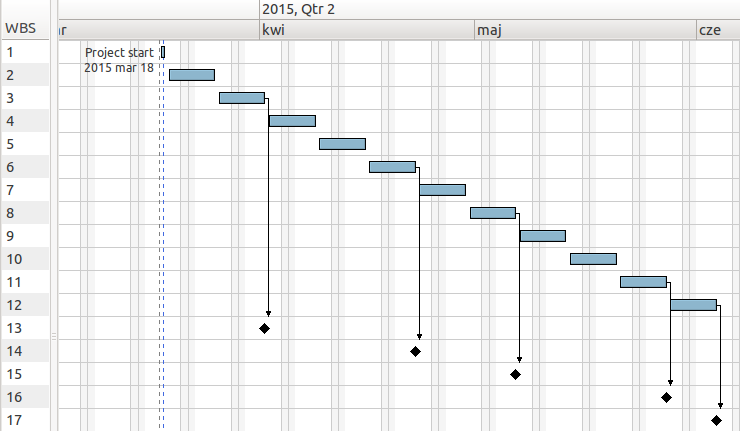
\includegraphics[width=\textwidth]{../harmonogram/gantt.png}
 \end{center}
 \caption{Diagram Gantta}
 \label{fig:gantt}
\end{figure}
 